\chapter{图上的行走}
\label{chap:graph-walks}

在图的一个顶点放下一枚棋子。每到一处，棋子按邻边的权重比例随机选一个邻居移过去。重复同样的试验——每次从同一个顶点出发，都走五步——统计五步后落在各点的比例，就能估计第五步的位置分布。

位置分布并不是唯一值得关心的问题。另一种问题是：首次到达某个指定顶点需要几步？还有一种更强的问题：把所有顶点都走到需要几步？它们固定的不是步数，而是停止条件，每次试验的步数都可能不同。

对于位置分布，一步选择写成矩阵乘法，多步演化由矩阵的幂给出。归一化拉普拉斯的谱可以判断分布是否最终收敛到平稳状态，并估计达到给定精度需要走多少步。对于等待时间，给目标顶点固定边界值后，首达期望满足接地拉普拉斯方程。往返等待时间还可以直接用有效电阻表示。

最后两节在有向图上加入重启。重启分布给出了行走中断后从哪里重新出发的偏好，由此得到PageRank排名。将重启集中在少数种子上，可以逐点推送尚未处理的概率质量，只访问种子附近的顶点。

除有向排名一节另作说明外，本章取正权支撑连通、至少有两个顶点的有限无向图。记$V$为顶点集，$n=|V|$为顶点数。顶点$i$的加权度为$d_i$，度向量为$\bm{d}=(d_1,\ldots,d_n)^\top$，度矩阵为$\bm{D}=\operatorname{diag}(d_1,\ldots,d_n)$。总加权度$\operatorname{vol}(V)=\sum_{i\in V}d_i$也叫全图的体积。概率分布写成行向量，顶点函数写成列向量。PageRank中的$\alpha\in(0,1)$始终表示重启概率，沿图转移的概率为$1-\alpha$。

\section{随机游走}
\label{sec:graph-random-walk}

一步怎样选邻居，决定了多步以后棋子可能落在哪里。我们先从四点路径上的具体走步出发，明确一步选择的规则，再将所有可能行走的终点汇总为位置分布。

\subsection{随机游走}
\label{sec:graph-walk-rule}

在单位权路径$1\!-\!2\!-\!3\!-\!4$上，把棋子放在顶点$1$。顶点$1$只有一条边连到$2$，所以第一步别无选择，必须走到$2$。

到了$2$之后，面前有两条边：一条回到$1$，一条通往$3$。两条边的权重都是$1$，总共$2$。回到$1$的概率是$1/2$，走到$3$的概率也是$1/2$。如果把从$2$到$3$的边权提高为$3$，那么从$2$离开时两条边的权重共为$1+3=4$，回到$1$的概率变成$1/4$，走到$3$的概率变成$3/4$。选择概率始终由出发顶点的邻边权重决定。

\begin{definition}[随机游走]
\label{def:graph-random-walk}
记$X_t$为第$t$步所在的顶点。给定$X_t=i$，下一步选择$j$的概率与边权$w_{i,j}$成正比，
\begin{equation}
\mathbb{P}(X_{t+1}=j\mid X_0,\ldots,X_t)=\frac{w_{i,j}}{d_i}.
\label{eq:graph-walk-transition-rule}
\end{equation}
若$d_i=0$（孤立顶点），约定棋子停留在原地。
\end{definition}

这条\term{随机游走}（random walk）规则只读取当前位置。即使两次走到$i$的路线完全不同，从$i$出发的下一步概率仍然一样。

用$\nu_i^{(t)}=\mathbb{P}(X_t=i)$记第$t$步在顶点$i$的概率，把各点的概率排成一行，记作$\bm{\nu}^{(t)}$。下标$i$指定顶点，上标$(t)$指定时刻。$\bm{\nu}^{(0)}$就是起点分布。

一条给定的行走序列$v_0,v_1,\ldots,v_k$要求棋子先出现在$v_0$，再依次完成各步转移。每接上一步，就把此前走完该前缀的概率乘上这一跳的转移概率。因此这条行走的概率为
\begin{equation}
\mathbb{P}(X_0=v_0,\ldots,X_k=v_k)
=\nu^{(0)}_{v_0}\prod_{j=0}^{k-1}\frac{w_{v_j,v_{j+1}}}{d_{v_j}}.
\label{eq:graph-walk-path-probability}
\end{equation}

回到单位权路径。从$1$出发，$1\to2\to1$的概率是$1\cdot(1/2)=1/2$，$1\to2\to3$的概率也是$1\cdot(1/2)=1/2$。两条路径走了相同的步数，但中途经过不同的顶点。若包含孤点，对应因子按停留规则取$1$。

\subsection{多步分布}
\label{sec:graph-walk-distributions}

上面计算了单条路径的概率。如果要问"第$t$步落在顶点$j$的概率是多少"，就需要把所有在第$t$步到达$j$的路径概率加起来。转移矩阵把这个求和变成一次矩阵乘法。

\paragraph{转移矩阵}

把从每个顶点出发的一步选择概率排成一行，再把$n$行叠起来，就得到\term{转移矩阵}（transition matrix）$\bm{P}$。第$i$行记录从$i$出发到各点的概率，第$j$列收集各处走到$j$的概率。设加权邻接矩阵为$\bm{W}=(w_{i,j})$，把$\bm{W}$的第$i$行除以$d_i$，等于在左侧乘$\bm{D}^{-1}$，于是
\begin{equation}
\bm{P}=\bm{D}^{-1}\bm{W}.
\label{eq:graph-walk-transition-matrix}
\end{equation}
矩阵元素非负，每行之和为$1$，即$\bm{P}\bm{1}=\bm{1}$。

\paragraph{一步更新}

要算第$t+1$步到达$j$的概率，可以按上一步所在的位置$i$分类。棋子在第$t$步落在$i$的概率是$\nu_i^{(t)}$，从$i$一步到$j$的概率是$P_{i,j}$。把这两个概率相乘再对所有$i$求和，就得到
\begin{equation}
\nu^{(t+1)}_j=\sum_i \nu^{(t)}_i P_{i,j}.
\label{eq:graph-walk-distribution-entry}
\end{equation}

这个求和就是概率行$\bm{\nu}^{(t)}$右乘$\bm{P}$的第$j$个分量。每多走一步，右边就多乘一个$\bm{P}$，从而
\begin{equation}
\bm{\nu}^{(t+1)}=\bm{\nu}^{(t)}\bm{P},
\qquad
\bm{\nu}^{(t)}=\bm{\nu}^{(0)}\bm{P}^t.
\label{eq:graph-walk-distribution}
\end{equation}
取初始分布为顶点$u$上的点质量，$\bm{P}^t$的第$u$行就是第$t$步的分布。

\paragraph{四点路径的前四步}

在单位权路径$1\!-\!2\!-\!3\!-\!4$上，四个顶点的度分别为$1,2,2,1$。转移矩阵为
\[
\bm{P}=\begin{pmatrix}
0&1&0&0\\
1/2&0&1/2&0\\
0&1/2&0&1/2\\
0&0&1&0
\end{pmatrix}.
\]
从顶点$1$出发，初始行只有第一个分量为$1$。第一次乘$\bm{P}$时，只读取$\bm{P}$的第一行，所以一步后全部质量集中在顶点$2$。

第二次乘$\bm{P}$时读取第二行。顶点$2$的$1/2$概率回到$1$，$1/2$概率走到$3$。第三次乘$\bm{P}$时，分别取$\bm{P}$的第一行和第三行各乘$1/2$再相加。包含初态的计算结果为
\[
\begin{array}{c@{\qquad}c}
t&\bm{\nu}^{(t)}\\
0&(1,0,0,0)\\
1&(0,1,0,0)\\
2&(1/2,0,1/2,0)\\
3&(0,3/4,0,1/4)
\end{array}
\]
图~\ref{fig:graph-walk-path-distribution}把各步连起来。顺着顶点$2$在$t=3$处接到的两条箭头往回看，$3/4$中有$1/2$来自顶点$1$（经路线$1\to2$），另有$1/4$来自顶点$3$（经路线$3\to2$）。

图~\ref{fig:graph-walk-bar-chart}以柱状图展示同一组分布。每个面板对应一个时刻，柱高是当前在各顶点的概率。观察概率如何从起点逐步向路径的另一端扩散：$t=1$时质量全部集中在$2$，$t=2$时分到$1$和$3$，$t=3$时已传到$4$。

\begin{figure}[!htb]
\centering
\begin{tikzpicture}[x=1mm,y=1mm,
  bar/.style={fill=FigureBlueFill,draw=FigureBlue,line width=.45pt},
  panel/.style={anchor=mid,font=\figurefont\footnotesize},
  vlabel/.style={font=\figurefont\fontsize{7.5}{9}\selectfont,FigureInk,anchor=north},
  plabel/.style={font=\figurefont\fontsize{7}{8.5}\selectfont,FigureInk,anchor=south}]
  \def\barw{4}
  \def\barscale{20}
  \def\gap{3}
  % Panel t=1: (0,1,0,0)
  \begin{scope}[xshift=0mm]
    \draw[FigureStroke,line width=.4pt] (0,0) -- (0,\barscale+2);
    \draw[FigureStroke,line width=.4pt] (0,0) -- (4*\barw+3*\gap+1,0);
    \foreach \i/\v/\p in {0/1/0, 1/2/1, 2/3/0, 3/4/0} {
      \pgfmathsetmacro{\x}{\i*(\barw+\gap)+1}
      \pgfmathsetmacro{\h}{\p*\barscale}
      \ifnum\p>0
        \fill[bar] (\x,0) rectangle +(\barw,\h);
        \node[plabel] at (\x+\barw/2,\h) {$\p$};
      \fi
      \node[vlabel] at (\x+\barw/2,-1) {$\v$};
    }
    \node[panel] at (16,-8) {(a) $t=1$};
  \end{scope}
  % Panel t=2: (1/2,0,1/2,0)
  \begin{scope}[xshift=38mm]
    \draw[FigureStroke,line width=.4pt] (0,0) -- (0,\barscale+2);
    \draw[FigureStroke,line width=.4pt] (0,0) -- (4*\barw+3*\gap+1,0);
    \foreach \i/\v/\p/\plbl in {0/1/0.5/{1/2}, 1/2/0/{}, 2/3/0.5/{1/2}, 3/4/0/{}} {
      \pgfmathsetmacro{\x}{\i*(\barw+\gap)+1}
      \pgfmathsetmacro{\h}{\p*\barscale}
      \pgfmathparse{\p>0?1:0}
      \ifnum\pgfmathresult=1
        \fill[bar] (\x,0) rectangle +(\barw,\h);
        \node[plabel] at (\x+\barw/2,\h) {$\plbl$};
      \fi
      \node[vlabel] at (\x+\barw/2,-1) {$\v$};
    }
    \node[panel] at (16,-8) {(b) $t=2$};
  \end{scope}
  % Panel t=3: (0,3/4,0,1/4)
  \begin{scope}[xshift=76mm]
    \draw[FigureStroke,line width=.4pt] (0,0) -- (0,\barscale+2);
    \draw[FigureStroke,line width=.4pt] (0,0) -- (4*\barw+3*\gap+1,0);
    \foreach \i/\v/\p/\plbl in {0/1/0/{}, 1/2/0.75/{3/4}, 2/3/0/{}, 3/4/0.25/{1/4}} {
      \pgfmathsetmacro{\x}{\i*(\barw+\gap)+1}
      \pgfmathsetmacro{\h}{\p*\barscale}
      \pgfmathparse{\p>0?1:0}
      \ifnum\pgfmathresult=1
        \fill[bar] (\x,0) rectangle +(\barw,\h);
        \node[plabel] at (\x+\barw/2,\h) {$\plbl$};
      \fi
      \node[vlabel] at (\x+\barw/2,-1) {$\v$};
    }
    \node[panel] at (16,-8) {(c) $t=3$};
  \end{scope}
\end{tikzpicture}
\caption{从顶点$1$出发在四点路径上的前三步位置分布。柱高表示当前在各顶点的概率。$t=1$时全部质量在$2$。$t=2$时分成两半回到$1$和前进到$3$。$t=3$时已到达端点$4$，但$3/4$的质量留在$2$。}
\label{fig:graph-walk-bar-chart}
\end{figure}

\begin{BookInlineFigure}
\centering
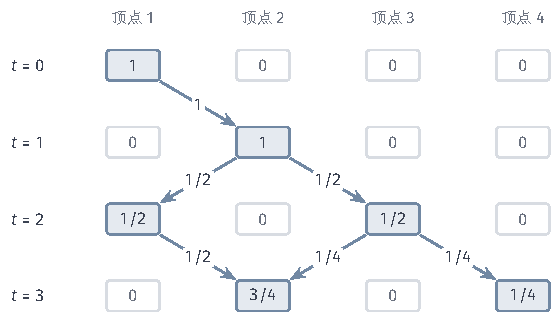
\includegraphics[width=94.132mm]{figures/03-graphs/05-matrices-and-spectra/tikz/walk-examples/path-distribution.pdf}
\caption{单位权路径$1\!-\!2\!-\!3\!-\!4$上从顶点$1$出发的分布。每行对应一个时刻，格内是当前位置的概率，箭头上的数字是这一小股概率在一步中实际转移的量。}
\label{fig:graph-walk-path-distribution}
\end{BookInlineFigure}

\paragraph{与邻接矩阵幂的关系}

第~\ref{chap:graph-adjacency-matrix}章用邻接矩阵$\bm{A}$的幂$(\bm{A}^t)_{u,v}$来计算从$u$到$v$的$t$步行走条数。在无权$d$正则图上，每个顶点的度都是$d$，每一步沿指定边行走的概率为$1/d$。同一条$t$步行走的概率为$d^{-t}$，因此
\[
\bm{P}^t=d^{-t}\bm{A}^t.
\]
度随顶点变化时，同样长的行走可有不同概率，上式不再成立。例如在四点路径上，从顶点$2$出发，$2\to1\to2$的概率是$(1/2)\cdot1=1/2$，$2\to3\to2$的概率是$(1/2)\cdot(1/2)=1/4$。两条路径长度相同，但经过不同度数的顶点，概率不一样。

\section{平稳分布}
\label{sec:graph-walk-stationary}

走了很多步以后，分布会不会停在某个固定形状上？如果给每个顶点分配一定的概率质量，使得一步转移后各点的质量恰好不变，这份分布就叫平稳分布。我们先用四点路径的具体算例看到这样的分布确实存在，再回到一般的无向图推导它的形式。

在四点路径上，试着给每条边的每个端点各分出$1/6$的质量。三条边共分出六份，各顶点收到的份数与自身的邻边数一致：端点$1$和$4$各收到一份，中间的$2$和$3$各收到两份。于是初始质量为$(1,2,2,1)/6$。

现在看一步转移。端点$1$的一份质量全部送给$2$。中间顶点$2$有两份质量，一份送给$1$，另一份送给$3$。边$23$和$34$上的情况也是类似的对称交换。图~\ref{fig:graph-walk-stationary-edge-balance}标出了每条边上的两笔对向转移。任取一个顶点，加起来的流入恰好等于加起来的流出。一步之后各点质量都没有变化。

\begin{BookInlineFigure}
\centering
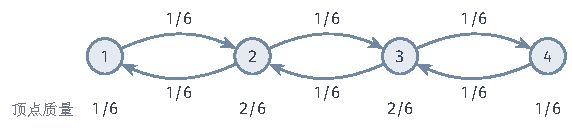
\includegraphics[width=96.936mm]{figures/03-graphs/05-matrices-and-spectra/tikz/walk-examples/stationary-edge-balance.pdf}
\caption{四顶点单位权路径的平稳概率及一步转移量。节点下方是原有质量，同一条边的两个方向各送出$1/6$。}
\label{fig:graph-walk-stationary-edge-balance}
\end{BookInlineFigure}

\begin{definition}[平稳分布]
\label{def:graph-walk-stationary}
若非负行向量$\bm{\pi}$满足$\sum_i\pi_i=1$且
\begin{equation}
\bm{\pi}\bm{P}=\bm{\pi},
\label{eq:graph-walk-stationary}
\end{equation}
则称$\bm{\pi}$是转移矩阵$\bm{P}$的\term{平稳分布}（stationary distribution）。
\end{definition}

上面四点路径的例子提示了一种做法：让每个顶点持有与其度成正比的质量。在一般的加权无向图上，令
\[
\pi_i=\frac{d_i}{\operatorname{vol}(V)}.
\]
下面验证这确实是一个平稳分布。

\paragraph{详细平衡}

考虑一条边$\{i,j\}$上的双向概率流。从$i$送往$j$的流量是当前在$i$的概率乘以从$i$到$j$的转移概率，
\[
\pi_i P_{i,j}=\frac{d_i}{\operatorname{vol}(V)}\cdot\frac{w_{i,j}}{d_i}
=\frac{w_{i,j}}{\operatorname{vol}(V)}.
\]
右边只含边权$w_{i,j}$，与方向无关。交换$i,j$后结果不变，因为$w_{i,j}=w_{j,i}$。这就是说，每条边上从两端送出的概率流相等。这个性质称为\term{详细平衡}（detailed balance）。

既然每条边的双向流已经抵消，对起点$i$求和后，流入$j$的总量自然等于$j$原有的质量$\pi_j$。因此按度分配的分布确实平稳。详细平衡是一个比平稳方程更强的条件：后者只要求每个顶点的总流入等于总流出，前者要求每条边上都各自平衡。

\paragraph{唯一性}

接下来说明连通无向图的平稳分布唯一。

\begin{theorem}[无向连通图的平稳分布]
\label{thm:graph-walk-stationary-uniqueness}
正权支撑连通的有限无向图的转移矩阵$\bm P$有唯一的平稳分布，且$\pi_i=d_i/\operatorname{vol}(V)$。
\end{theorem}

\begin{proof}
设$\bm{q}$是任意一个平稳分布，满足$\bm{q}\bm{P}=\bm{q}$。将等式写成$\bm{q}\bm{D}^{-1}\bm{W}=\bm{q}$，两边转置得
\[
\bm{W}\bm{D}^{-1}\bm{q}^\top=\bm{q}^\top.
\]
这里用了$\bm{W}$对称和$\bm{D}^{-1}$为对角矩阵。

令$\bm{y}=\bm{D}^{-1}\bm{q}^\top$，即$y_i=q_i/d_i$。等式右边的$\bm{q}^\top$可以写成$\bm{D}\bm{y}$，于是
\[
(\bm{D}-\bm{W})\bm{y}=\bm{0}.
\]
左边正是组合拉普拉斯$\bm{L}$作用于$\bm{y}$。第~\ref{chap:graph-laplacian-matrix}章指出，连通图的拉普拉斯零空间由常向量张成。这意味着$y_i=q_i/d_i$对所有$i$取相同的值。由总质量$\sum_i q_i=1$确定这个常数为$1/\operatorname{vol}(V)$，于是
\begin{equation}
\pi_i=\frac{d_i}{\operatorname{vol}(V)}.
\label{eq:graph-walk-stationary-degrees}
\end{equation}
\end{proof}

\paragraph{不连通与收敛的区别}

若图有多个正权连通分量，每个分量可以独立保有自己的概率质量。取各分量平稳分布的任意凸组合仍然平稳，因此唯一性不再成立。孤点上的点质量也可以保留——在停留规则下它已经平稳。

回到只有一条边的两点图。它只有一个正权分量，平稳分布唯一，为$(1/2,1/2)$。但如果从其中一个顶点出发，棋子每一步切换顶点，分布在$(1,0)$与$(0,1)$之间交替，始终不收敛。平稳分布的唯一性回答了"哪些分布保持不变"，至于任意初态能否到达它，还需要检查矩阵幂的行为。

\section{收敛速度}
\label{sec:graph-walk-convergence}

上一节末尾看到，在二部图上单点出发的随机游走会永久奇偶振荡。对于一般的连通无向图，从任意初态$\bm\nu^{(0)}$出发的多步分布$\bm\nu^{(t)}=\bm\nu^{(0)}\bm P^t$究竟何时收敛到平稳分布$\bm\pi$？如果收敛，需要走多少步才能与平稳分布足够接近？本节先将转移矩阵$\bm P$对称化以对接归一化拉普拉斯谱，再导出收敛的充要条件与误差衰减界，最后对比几类典型图的收敛速度。

\subsection{转移矩阵的对称化}
\label{sec:graph-walk-symmetrization}

在度数不均匀的无向图上，虽然边权对称（$w_{i,j}=w_{j,i}$），转移矩阵$\bm P=\bm D^{-1}\bm W$本身通常并\emph{不对称}（例如在四点路径上，$P_{1,2}=1$而$P_{2,1}=1/2$）。为了使用实对称矩阵的正交谱分解，我们对$\bm P$作度平方根相似变换：将第$i$行乘以$\sqrt{d_i}$、第$j$列除以$\sqrt{d_j}$，其$(i,j)$元变为对称的$\frac{w_{i,j}}{\sqrt{d_i d_j}}$。写成矩阵形式，即左乘$\bm D^{1/2}$、右乘$\bm D^{-1/2}$：
\begin{equation}
\bm{S}=\bm{D}^{1/2}\bm{P}\bm{D}^{-1/2}
=\bm{D}^{-1/2}\bm{W}\bm{D}^{-1/2}=\bm{I}-\mathcal{L},
\label{eq:graph-walk-symmetric-transition}
\end{equation}
其中$\mathcal L=\bm D^{-1/2}\bm L\bm D^{-1/2}$正是第~\ref{sec:graph-normalized-laplacian}节的对称归一化拉普拉斯矩阵。

式~\eqref{eq:graph-walk-symmetric-transition}建立起了随机游走与归一化拉普拉斯谱之间的直接桥梁：
\begin{enumerate}
\item \emph{特征值一一对应}：因为$\bm P=\bm D^{-1/2}\bm S\bm D^{1/2}$与实对称矩阵$\bm S$相似，两者的特征值完全相同。设$\mathcal L$的特征值按升序排列为$0=\mu_1<\mu_2\leq\cdots\leq\mu_n\leq 2$，则$\bm P$与$\bm S$的特征值按降序排列为
\[
  1=\theta_1>\theta_2\geq\cdots\geq\theta_n\geq -1,
  \qquad \theta_i = 1 - \mu_i.
\]
\item \emph{多步演化的对称坐标表示}：由$\bm P\bm D^{-1/2}=\bm D^{-1/2}\bm S$，在多步演化式$\bm\nu^{(t+1)}=\bm\nu^{(t)}\bm P$两侧右乘$\bm D^{-1/2}$，可得
\[
\bm{\nu}^{(t+1)}\bm{D}^{-1/2}
=(\bm{\nu}^{(t)}\bm{D}^{-1/2})\bm{S}
=(\bm{\nu}^{(0)}\bm{D}^{-1/2})\bm{S}^{t+1}.
\]
也就是说，只要把概率分布行向量$\bm\nu^{(t)}$缩放为$\bm\nu^{(t)}\bm D^{-1/2}$，每走一步就等价于右乘一次实对称矩阵$\bm S$。
\end{enumerate}

例如在单位权四点路径上，$\bm P$与$\bm S$的四个特征值为$\{1,\frac12,-\frac12,-1\}$；在单位权四元环$C_4$上，特征值为$\{1,0,0,-1\}$。两者的最小特征值都达到了$-1$（对应$\mu_4=2$）。

\subsection{收敛条件}
\label{sec:graph-walk-convergence-condition}

利用对称矩阵$\bm S$的标准正交特征基，可以一步写出第$t$步分布$\bm\nu^{(t)}$与平稳分布$\bm\pi$之间的偏差演化公式。

设$\bm u_1,\bm u_2,\ldots,\bm u_n$为$\bm S$对应于$1=\theta_1>\theta_2\geq\cdots\geq\theta_n\geq -1$的标准正交特征向量（列向量），其中第一特征向量为$\bm u_1=\bm D^{1/2}\bm 1/\sqrt{\operatorname{vol}(V)}$。记第$t$步的分布偏差行向量为$\bm z^{(t)}=\bm\nu^{(t)}-\bm\pi$。由于$\bm\nu^{(t)}\bm 1=1$且$\bm\pi\bm 1=1$，偏差的分量和恒为零：$\bm z^{(t)}\bm 1=0$。因此在对称坐标下，缩放偏差$\bm z^{(t)}\bm D^{-1/2}$与第一特征向量$\bm u_1$恒正交：
\[
(\bm z^{(t)}\bm D^{-1/2})\bm u_1
=\frac{1}{\sqrt{\operatorname{vol}(V)}}(\bm z^{(t)}\bm D^{-1/2})(\bm D^{1/2}\bm 1)
=\frac{\bm z^{(t)}\bm 1}{\sqrt{\operatorname{vol}(V)}}=0.
\]
这意味着偏差在$\bm u_1$方向上的分量恒为$0$。将初始缩放偏差在其余$n-1$个非平稳特征方向$\bm u_2,\ldots,\bm u_n$上展开为$\bm z^{(0)}\bm D^{-1/2}=\sum_{i=2}^n a_i\bm u_i^\top$（其中$a_i=\bm z^{(0)}\bm D^{-1/2}\bm u_i$），每走一步右乘$\bm S$就将第$i$项乘上$\theta_i$，从而第$t$步的缩放偏差精确等于
\begin{equation}
\bm{z}^{(t)}\bm{D}^{-1/2}
=\sum_{i=2}^n a_i\theta_i^t\bm{u}_i^\top.
\label{eq:graph-walk-spectral-evolution}
\end{equation}

\begin{theorem}[无向连通图随机游走的收敛判别]
\label{thm:graph-walk-convergence}
设有限无向图的正权支撑连通且至少有两个顶点，平稳分布为$\bm\pi$。则从任意初始分布$\bm\nu^{(0)}$出发的随机游走分布$\bm\nu^{(t)}=\bm\nu^{(0)}\bm P^t$当$t\to\infty$时收敛于$\bm\pi$，当且仅当正权支撑不是二部图（等价于最小特征值$\theta_n>-1$，或$\mu_n<2$）。
\end{theorem}

\begin{proof}
由式~\eqref{eq:graph-walk-spectral-evolution}及$\bm u_2,\ldots,\bm u_n$的标准正交性，有$\lVert\bm z^{(t)}\bm D^{-1/2}\rVert_2^2=\sum_{i=2}^n a_i^2\theta_i^{2t}$。该平方和在$t\to\infty$时对任意初始系数$(a_2,\ldots,a_n)$趋于$0$，当且仅当对所有$i=2,\ldots,n$都有$|\theta_i|<1$。由于连通图上$1>\theta_2\geq\cdots\geq\theta_n\geq -1$，故$\max_{i\geq 2}|\theta_i|<1$当且仅当$\theta_n>-1$（即$\mu_n=1-\theta_n<2$）。由第~\ref{sec:graph-normalized-laplacian}节定理~\ref{prop:graph-normalized-spectrum-bound}，这等价于图不是二部图。必要性并不要求任意系数组合都能表示概率分布：若存在$\theta_i=-1$，可取$\bm\nu^{(0)}=\bm\pi+a\bm u_i^\top\bm D^{1/2}$，其中非零$a$足够小。其分量和为$1$且逐项非负，却保留不衰减的交替模态。
\end{proof}

图~\ref{fig:graph-walk-parity}直观对比了非二部图与二部图的演化差异：在三角形$C_3$（非二部图，$\theta_2=\theta_3=-1/2$）上，偏差按$(-1/2)^t$指数衰减，分布迅速趋向均匀平稳分布；而在四元环$C_4$（二部图，$\theta_4=-1$）上，$\theta_4=-1$对应的正负交替模态$(-1)^t\bm u_4^\top$永不衰减，概率质量在奇偶两侧顶点集之间无休止地来回跳动。

\begin{figure}[!htb]
\centering
% Exact transient probabilities on the unweighted triangle and four-cycle.
\begin{tikzpicture}[x=1mm,y=1mm,font=\figurefont\fontsize{8}{9}\selectfont]
  \foreach \column/\step in {0/0,1/1,2/2,3/3} {
    \node[text=FigureInk] at ({20*\column+8},35) {$t=\step$};
  }
  \node[anchor=east,text=FigureInk] at (-2,25) {$C_3$};
  \node[anchor=east,text=FigureInk] at (-2,7) {$C_4$};
  \foreach \column/\values in {0/{12,0,0},1/{0,6,6},2/{6,3,3},3/{3,4.5,4.5}} {
    \begin{scope}[shift={({20*\column},19)}]
      \foreach \value [count=\vertex from 1] in \values {
        \fill[FigureBlue] ({4*\vertex-2},0) rectangle ({4*\vertex+1},\value);
        \node[anchor=north,text=FigureInk] at ({4*\vertex-.5},0) {$\vertex$};
      }
      \draw[FigureStroke,line width=.55pt] (0,0)--(17.5,0);
      \draw[FigureStroke,dashed,line width=.55pt] (0,4)--(17.5,4);
    \end{scope}
  }
  \foreach \column/\values in {0/{12,0,0,0},1/{0,6,0,6},2/{6,0,6,0},3/{0,6,0,6}} {
    \begin{scope}[shift={({20*\column},1)}]
      \foreach \value [count=\vertex from 1] in \values {
        \fill[FigureBlue] ({4*\vertex-2},0) rectangle ({4*\vertex+1},\value);
        \node[anchor=north,text=FigureInk] at ({4*\vertex-.5},0) {$\vertex$};
      }
      \draw[FigureStroke,line width=.55pt] (0,0)--(17.5,0);
      \draw[FigureStroke,dashed,line width=.55pt] (0,3)--(17.5,3);
    \end{scope}
  }
\end{tikzpicture}

\caption{从顶点$1$出发的前四个时刻位置分布对比。每个面板自左至右以柱高表示各顶点的概率，水平虚线为均匀平稳概率。三角形$C_3$（上排）按$(-1/2)^t$迅速衰减收敛；四元环$C_4$（下排）因含$\theta_4=-1$模态，质量始终在二部划分的两侧之间交替跳动。}
\label{fig:graph-walk-parity}
\end{figure}

\subsection{收敛速度}
\label{sec:graph-walk-lazy}

当随机游走满足收敛条件时，非平稳特征值的最大模长
\[
  \rho = \max_{2\leq i\leq n}|\theta_i| = \max\{\theta_2, -\theta_n\} < 1
\]
直接决定了偏差$\bm z^{(t)}=\bm\nu^{(t)}-\bm\pi$向零衰减的几何速率，而$1-\rho>0$则称为转移矩阵的\term{绝对谱隙}（absolute spectral gap）。

\paragraph{总变差距离与谱间隙衰减界}

为了定量衡量第$t$步分布$\bm\nu^{(t)}$与平稳分布$\bm\pi$的接近程度，概率论中标准采用\term{总变差}（total variation）距离：
\[
  \lVert\bm\nu-\bm\pi\rVert_{\mathrm{TV}}
  =\frac12\lVert\bm\nu-\bm\pi\rVert_1
  =\frac12\sum_{i=1}^n|\nu_i-\pi_i|
  =\max_{A\subseteq V}\bigl|\bm\nu(A)-\bm\pi(A)\bigr|.
\]
另一方面，在对称坐标式~\eqref{eq:graph-walk-spectral-evolution}中，最契合正交展开的欧氏范数是以平稳概率$\pi_i=d_i/\operatorname{vol}(V)$倒数加权的$\pi^{-1}$-范数：
\[
\lVert\bm{z}\rVert_{\pi^{-1}}^2
=\sum_{i=1}^n\frac{z_i^2}{\pi_i}
=\operatorname{vol}(V)\,\lVert\bm{z}\bm{D}^{-1/2}\rVert_2^2.
\]
下面的定理通过Cauchy--Schwarz不等式将两者衔接，给出总变差距离随步数$t$的指数衰减上界。

\begin{theorem}[谱间隙与总变差收敛速度]
\label{prop:graph-walk-tv-bound}
设连通正权无向图随机游走的非平稳特征值最大模长为$\rho=\max_{i\geq 2}|\theta_i|$。则对任意初始分布$\bm\nu^{(0)}$及任意步数$t\geq 0$，有
\begin{equation}
\lVert\bm{\nu}^{(t)}-\bm{\pi}\rVert_{\pi^{-1}}
\le\rho^t\lVert\bm{\nu}^{(0)}-\bm{\pi}\rVert_{\pi^{-1}},
\qquad
\lVert\bm{\nu}^{(t)}-\bm{\pi}\rVert_{\mathrm{TV}}
\le\frac12\rho^t\lVert\bm{\nu}^{(0)}-\bm{\pi}\rVert_{\pi^{-1}}.
\label{eq:graph-walk-weighted-contraction}
\end{equation}
特别地，若从单个顶点$u\in V$确定性出发（$\bm\nu^{(0)}=\bm e_u^\top$），则
\begin{equation}
\lVert\bm{\nu}^{(t)}-\bm{\pi}\rVert_{\mathrm{TV}}
\le\frac12\sqrt{\frac{1}{\pi_u}-1}\;\rho^t.
\label{eq:graph-walk-tv-bound}
\end{equation}
\end{theorem}

\begin{proof}
记$\bm z^{(t)}=\bm\nu^{(t)}-\bm\pi$。由正交展开式~\eqref{eq:graph-walk-spectral-evolution}，有
\[
\lVert\bm{z}^{(t)}\bm{D}^{-1/2}\rVert_2^2
=\sum_{i=2}^n a_i^2|\theta_i|^{2t}
\le \rho^{2t}\sum_{i=2}^n a_i^2
=\rho^{2t}\lVert\bm{z}^{(0)}\bm{D}^{-1/2}\rVert_2^2.
\]
两边同乘$\operatorname{vol}(V)$并开方即得式~\eqref{eq:graph-walk-weighted-contraction}第一式。接着将$|z_i^{(t)}|$分解为$\sqrt{\pi_i}\cdot\frac{|z_i^{(t)}|}{\sqrt{\pi_i}}$，应用Cauchy--Schwarz不等式并利用$\sum_{i=1}^n\pi_i=1$，得
\[
2\lVert\bm z^{(t)}\rVert_{\mathrm{TV}}
=\sum_{i=1}^n|z_i^{(t)}|
\le\left(\sum_{i=1}^n\pi_i\right)^{1/2}
   \left(\sum_{i=1}^n \frac{(z_i^{(t)})^2}{\pi_i}\right)^{1/2}
=\lVert\bm{z}^{(t)}\rVert_{\pi^{-1}}
\le\rho^t\lVert\bm{z}^{(0)}\rVert_{\pi^{-1}},
\]
同除以$2$即得式~\eqref{eq:graph-walk-weighted-contraction}第二式。当$\bm\nu^{(0)}=\bm e_u^\top$时，$z_u^{(0)}=1-\pi_u$，对$j\neq u$有$z_j^{(0)}=-\pi_j$，故$\lVert\bm z^{(0)}\rVert_{\pi^{-1}}^2=\frac{(1-\pi_u)^2}{\pi_u}+(1-\pi_u)=\frac{1}{\pi_u}-1$，代入即得式~\eqref{eq:graph-walk-tv-bound}。
\end{proof}

由式~\eqref{eq:graph-walk-tv-bound}可知，要使总变差距离降低到给定精度$0<\varepsilon<1/2$以内，利用$\rho^t=(1-(1-\rho))^t\leq\mathrm e^{-(1-\rho)t}$，定义\term{混合时间}（mixing time）为使所有单点初态的总变差误差均不超过$\varepsilon$的最小非负整数时刻。记$\pi_{\min}=\min_i\pi_i$，在$\rho<1$时，上述界给出
\begin{equation}
  t_{\mathrm{mix}}(\varepsilon) \leq \left\lceil\frac{1}{1-\rho}\log\frac{1}{2\varepsilon\sqrt{\pi_{\min}}}\right\rceil.
  \label{eq:graph-walk-mixing-time-bound}
\end{equation}
这一充分步数上界包含$(1-\rho)^{-1}$，同时依赖目标误差与$\pi_{\min}$；它不是实际混合时间与谱隙的精确反比关系。

\paragraph{惰性游走：消除负特征值振荡}

在二部图或接近二部图的网络中，最小特征值$\theta_n\approx -1$会导致$\rho=\max\{\theta_2,-\theta_n\}$由高频奇偶振荡项$-\theta_n$主导。为使转移矩阵的全部特征值非负，算法应用中常采用\term{惰性游走}（lazy random walk）：每一步先抛一枚公平硬币，以$1/2$的概率停留在当前顶点不动，以$1/2$的概率按原转移矩阵$\bm P$走一步。惰性游走的转移矩阵为
\begin{equation}
\bm{Q}=\frac{\bm{I}+\bm{P}}{2}=\bm I - \frac12\bm L_{\mathrm{rw}}.
\label{eq:graph-walk-lazy-transition}
\end{equation}
由于原地停留和按$\bm P$转移都保持$\bm\pi$不变，惰性游走具有完全相同的平稳分布$\bm\pi$；但它的特征值被平移缩放为$\theta_i(\bm Q)=\frac{1+\theta_i}{2}=1-\frac{\mu_i}{2}\in[0,1]$，全部变为非负实数。此时原先$\theta_n=-1$的奇偶振荡模态直接变为$0$，非平稳特征值的最大模长完全由归一化拉普拉斯的第二小特征值$\mu_2$决定：
\[
  \rho(\bm Q) = 1 - \frac{\mu_2}{2},
  \qquad
  \text{惰性谱隙 } \gamma = 1 - \rho(\bm Q) = \frac{\mu_2}{2}.
\]

\subsection{典型图的收敛速度}
\label{sec:graph-walk-bottleneck}

将上一小节的惰性谱隙$\gamma=\mu_2/2$与第~\ref{sec:graph-cheeger}节的Cheeger不等式$\frac{\mu_2}{2}\leq\phi_*\leq\sqrt{2\mu_2}$结合，立即可得谱隙$\gamma$与全图最小导通率$\phi_*$的双向控制关系：
\begin{equation}
\frac{\phi_*^2}{4}\le\gamma\le\phi_*.
\label{eq:graph-walk-lazy-cheeger}
\end{equation}
式~\eqref{eq:graph-walk-lazy-cheeger}从几何上解释了什么图收敛快、什么图收敛慢：当$\operatorname{vol}(S)\leq\operatorname{vol}(V)/2$时，普通游走的导通率$\phi(S)=\frac{c(S,\bar S)}{\operatorname{vol}(S)}$正是平稳状态下棋子位于集合$S$内时“下一步跨过边界离开$S$的条件概率”；如果图中存在导通率$\phi_*$极小的稀疏割瓶颈，棋子一旦落入瓶颈一侧就很难穿过狭窄的咽喉逃到另一侧，谱隙$\gamma\leq\phi_*$必然极小，混合时间随之急剧拉长。

下面固定总变差误差$0<\varepsilon<1/2$，比较四类图族的谱隙与混合时间。除明确说明的普通游走外，均使用惰性游走；典型量级中的常数可以依赖$\varepsilon$。

\paragraph{1. 完全图$K_n$（固定误差下常数步混合，$t_{\mathrm{mix}}=\Theta(1)$）}

在单位权完全图$K_n$上（$n\geq3$），归一化拉普拉斯的所有非零特征值均为$\mu_2=\cdots=\mu_n=\frac{n}{n-1}>1$。普通游走的非平稳特征值全为$\theta_i=-\frac{1}{n-1}$，谱半径$\rho=\frac{1}{n-1}$随$n$增大反而趋于$0$；即便采用惰性游走，谱隙也高达$\gamma=\frac{n}{2(n-1)}>\frac12$。从任意顶点出发，仅需$O(1)$步即可在整个完全图上接近均匀分布。

\paragraph{2. 超立方体$Q_d$（对数级快速混合，$t_{\mathrm{mix}}=\Theta(d\log d)=\Theta(\log n\log\log n)$）}

在顶点数$n=2^d$的$d$维超立方体$Q_d$上，最小导通率为$\phi_*=1/d$，归一化第二小特征值为$\mu_2=2/d$（第~\ref{sec:graph-cheeger-tightness}小节）。惰性游走的谱隙为$\gamma=\frac{1}{d}=\frac{1}{\log_2 n}$。代入式~\eqref{eq:graph-walk-mixing-time-bound}（其中$\pi_u=2^{-d}$给出$\log(1/\sqrt{\pi_u})=\Theta(d)$），可知混合时间为$O(d^2)$（进一步利用坐标更新过程的耦合与谱展开可证明$t_{\mathrm{mix}}=\Theta(d\log d)$），虽然顶点数呈指数增长，随机游走却能在多项式对数步内迅速混合。

\paragraph{3. 路径图$P_n$与环图$C_n$（二次方扩散混合，$t_{\mathrm{mix}}=\Theta(n^2)$）}

在$n$点路径$P_n$或环$C_n$上，最小导通率为$\phi_*=\Theta(1/n)$，而归一化第二小特征值为$\mu_2=1-\cos(\Theta(1/n))=\Theta(n^{-2})$，惰性谱隙仅为$\gamma=\Theta(n^{-2})$。远离端点时，游走的位移呈扩散尺度，经过$t$步的典型距离为$O(\sqrt t)$，这解释了跨越长度$n$为何需要二次方时间。端点反射和惰性停留需另行计入；严格的$\Theta(n^2)$混合界可由路径、环的转移谱展开得到，不能只由单步方差推出。

\paragraph{4. 杠铃图（细腰瓶颈严重拖慢混合，$t_{\mathrm{mix}}=\Omega(n^2)$）}

将两个各含$k=n/2$个顶点的完全图$K_k$用一条单位权桥边相连（图~\ref{fig:graph-connectivity-archetypes}b）。虽然团内的位置分布在常数步内就可接近均匀，但单侧团的体积高达$\operatorname{vol}(S)=k(k-1)+1=\Theta(n^2)$，而跨桥割权仅为$c(S,\bar S)=1$，导致最小导通率骤降至
\[
  \phi_* = \frac{1}{k(k-1)+1} = \Theta(n^{-2}).
\]
由式~\eqref{eq:graph-walk-lazy-cheeger}的上界$\gamma\leq\phi_*=\Theta(n^{-2})$可知，这条细腰单桥构成了严重的扩散瓶颈：从团内平稳条件分布出发跨越桥边的等待具有$\Theta(n^2)$量级；谱隙的倒数也为混合时间提供相应下界，从而固定误差下全局混合时间为$\Omega(n^2)$。

\section{首达时间}
\label{sec:graph-walk-hitting}

前面固定时刻，考察棋子落在何处。现在换一个角度：固定目的地，问棋子在第几步首次到达。每次行走可能走不同的步数。我们先把这个步数当作一个随机量，再计算它的期望。

\subsection{首达期望的方程}
\label{sec:graph-walk-hitting-equation}

在四点路径上从顶点$1$出发，目标是$4$。一种可能是直走三步$1\to2\to3\to4$，另一种可能是走了五步$1\to2\to1\to2\to3\to4$，还有更长的情况。$\tau_4$记录的是某一次试验中实际走出的步数，$h_{1,4}$则是对所有可能步数按概率求出的平均值。

若起点已经是目标，一步也不用走。一般地，对目标$j$定义\term{首达时间}（hitting time）$\tau_j$，并用$h_{i,j}$表示从$i$出发的首达期望，
\begin{equation}
\tau_j=\inf\{t\ge0:X_t=j\},
\qquad h_{i,j}=\mathbb{E}_i[\tau_j].
\label{eq:graph-walk-hitting-definition}
\end{equation}
$\mathbb{E}_i$表示固定$X_0=i$后的期望，且$h_{j,j}=0$。

先检查期望是否有限。对每个非目标顶点选一条通往$j$的简单路径，长度至多$n-1$。沿这些路径逐步走完的最小概率为某个$p>0$。

将行走按每$n-1$步分块。不论上一块结束在什么位置，只要尚未到达目标，下一块命中它的概率至少为$p$。连续$k$块均未命中的概率至多$(1-p)^k$，几何级数求和给出等待的块数期望不超过$1/p$。每块最多$n-1$步，因此$h_{i,j}\le(n-1)/p$。

\paragraph{首步分解}

从$i\ne j$出发，第一步总要花一步。若这一步走到$k$，剩余等待时间的期望正是$h_{k,j}$，因为以后的转移只取决于当前位置。按第一步的去向加权求和，得到
\begin{equation}
h_{i,j}=1+\sum_k P_{i,k}h_{k,j},\qquad i\ne j.
\label{eq:graph-walk-first-step}
\end{equation}

\paragraph{化为拉普拉斯方程}

用$P_{i,k}=w_{i,k}/d_i$代入上式并两边乘$d_i$，一步的代价$1$变成$d_i$，
\[
d_i h_{i,j}-\sum_k w_{i,k}h_{k,j}=d_i,\qquad i\ne j.
\]
左边正是$\bm{D}-\bm{W}=\bm{L}$作用于首达期望列$\bm{h}_{:,j}$的第$i$个分量。

目标点$j$的分量已经固定为零，乘它的项都消失，因此删掉对应列。$j$处用的是边界条件$h_{j,j}=0$而非一步递推，因此也删掉相应行。记$-j$表示去掉坐标$j$，方程变为
\begin{equation}
\bm{L}_{-j,-j}\bm{h}_{-j,j}=\bm{d}_{-j}.
\label{eq:graph-walk-grounded-hitting}
\end{equation}
这正是第~\ref{sec:graph-laplacian-solve}节的接地系统。右端是度向量，因为乘以$d_i$把"走一步"的代价换算到拉普拉斯的尺度。

\paragraph{四点路径上的消元}

在单位权路径$1\!-\!2\!-\!3\!-\!4$上以$4$为目标。端点$1$的度为$1$，内点$2,3$的度为$2$。逐点写出方程，

从$1$出发：下一步必在$2$，故$h_{1,4}=1+h_{2,4}$。

从$2$出发：第一步以各$1/2$概率到$1$或$3$，故$h_{2,4}=1+(h_{1,4}+h_{3,4})/2$。

从$3$出发：一半概率到$2$，另一半概率到$4$（目标），故$h_{3,4}=1+h_{2,4}/2$。

乘上各点的度并移项，得到
\[
\begin{aligned}
h_{1,4}-h_{2,4}&=1,\\
-h_{1,4}+2h_{2,4}-h_{3,4}&=2,\\
-h_{2,4}+2h_{3,4}&=2.
\end{aligned}
\]
将第一式代入第二式，得到$h_{2,4}-h_{3,4}=3$。代回第三式得到$h_{3,4}=5$，逐项回代有
\[
\bm{h}_{:,4}=(9,8,5,0)^\top.
\]
图~\ref{fig:graph-walk-hitting-target}画出从$3$出发的两种第一步。两边各占一半加上必走的一步，得到$1+(8+0)/2=5$。

\begin{BookInlineFigure}
\centering
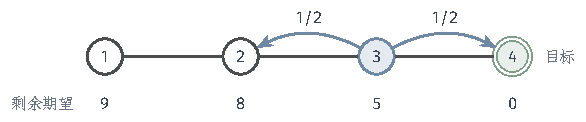
\includegraphics[width=99.24mm]{figures/03-graphs/05-matrices-and-spectra/tikz/walk-examples/hitting-path-target.pdf}
\caption{四顶点单位权路径以$4$为目标。节点下方是以该点为起点还要走的期望步数。箭头标出从$3$出发的两个去处及其概率，双圈标出目标。}
\label{fig:graph-walk-hitting-target}
\end{BookInlineFigure}

\paragraph{两个方向的首达期望不同}

从$1$到$2$只需一步。反过来从$2$到$1$就不一样了：$2$有$1/2$的概率直接到$1$，另有$1/2$的概率先走到$3$。走到$3$之后，要先从$3$绕回$2$，然后再重新尝试。

先算从$3$到$2$的平均时间。从$3$出发，$1/2$概率一步到$2$，$1/2$概率走到$4$。走到$4$后下一步必回$3$，等于白走两步回到原处。因此
\[
h_{3,2}=\tfrac{1}{2}\cdot1+\tfrac{1}{2}(2+h_{3,2}).
\]
解得$h_{3,2}=3$。

回到从$2$到$1$的问题。$1/2$概率一步到达，$1/2$概率先到$3$（一步），再从$3$回到$2$（平均$3$步），然后重新开始，
\[
h_{2,1}=\tfrac{1}{2}\cdot1+\tfrac{1}{2}(1+3+h_{2,1}).
\]
解得$h_{2,1}=5$。虽然$\{1,2\}$是一条无向边，但从两端出发绕远的机会完全不同。

在完全图$K_n$上，只要尚未命中目标，从任何非目标顶点出发，下一步命中的概率都是$1/(n-1)$。等待步数的期望就是$n-1$。

\subsection{往返时间与有效电阻}
\label{sec:graph-walk-commute-resistance}

从$i$去$j$再从$j$回$i$，总等待时间由两段组成。前一段的期望是$h_{i,j}$。前一段结束时，棋子恰好在$j$，此后每一步仍按相同规则转移，返程的条件期望都是$h_{j,i}$。两段相加，\term{往返时间}（commute time）的期望为$h_{i,j}+h_{j,i}$。

单向首达期望不对称。为了找到一个对称的表达式，先把首达方程恢复成全图形式。

将$\bm{L}\bm{h}_{:,j}$的各分量相加。$\bm{L}$的每一列和为零，因此总和也为零。已知$i\ne j$时第$i$项等于$d_i$，所以第$j$项必须抵消其余各项之和，等于$d_j-\operatorname{vol}(V)$。用$\bm{e}_j$记第$j$项为$1$、其余为$0$的列向量，全图方程为
\begin{equation}
\bm{L}\bm{h}_{:,j}=\bm{d}-\operatorname{vol}(V)\bm{e}_j.
\label{eq:graph-walk-full-hitting}
\end{equation}

右端各分量和为零，可以用伪逆$\bm{L}^\dagger$先求一个解。$\bm{L}^\dagger\bm{e}_j$取出伪逆的第$j$列，因此
\[
\bm{x}=\bm{L}^\dagger\bm{d}-\operatorname{vol}(V)\bm{L}^\dagger\bm{e}_j.
\]
这个解的第$j$项未必为零。由$\bm{L}\bm{1}=\bm{0}$，可以统一减去$x_j$后仍满足方程，同时保证$h_{j,j}=0$。展开$h_{i,j}=x_i-x_j$，得
\begin{equation}
h_{i,j}=(\bm{L}^\dagger\bm{d})_i-(\bm{L}^\dagger\bm{d})_j
+\operatorname{vol}(V)
\bigl((\bm{L}^\dagger)_{j,j}-(\bm{L}^\dagger)_{i,j}\bigr).
\label{eq:graph-walk-hitting-pseudoinverse}
\end{equation}
第一行包含度向量的信息，记录了度分配对单向首达时间的影响。正则图上度为常向量，这一部分消失。

把去程和返程相加。交换$i,j$后，第一行的两个差值恰好符号相反，抵消为零。剩下的是总加权度乘
\[
(\bm{L}^\dagger)_{i,i}+(\bm{L}^\dagger)_{j,j}
-(\bm{L}^\dagger)_{i,j}-(\bm{L}^\dagger)_{j,i}.
\]
把差向量$\bm{e}_i-\bm{e}_j$放在$\bm{L}^\dagger$的两侧相乘，展开后恰好是这四项。这正是第~\ref{sec:graph-effective-resistance}节的有效电阻二次型。

\begin{theorem}[往返时间与有效电阻]
\label{thm:graph-walk-commute-resistance}
对正权支撑连通的有限无向图，任意两点$i,j$的往返期望为
\begin{equation}
h_{i,j}+h_{j,i}
=\operatorname{vol}(V)\,R_{i,j}.
\label{eq:graph-walk-commute-time}
\end{equation}
\end{theorem}

有效电阻衡量一对顶点间的电势响应，乘以总加权度后就给出两次首达所需的平均总步数。

在四点路径上，总加权度为$1+2+2+1=6$。相邻点$1,2$之间只有一条单位电阻边，$R_{1,2}=1$，往返期望为$6$，与$h_{1,2}+h_{2,1}=1+5$一致。两端之间串联三条边，$R_{1,4}=3$，往返期望为$18$，即两个方向各$9$步。

在$n$点单位权环上，若两点沿环相隔$k$条边，两段弧的电阻分别为$k$和$n-k$，并联后得到$R=k(n-k)/n$。总度为$2n$，往返期望为$2k(n-k)$。

若把所有电导同时乘$c>0$，每步用边权除以度，转移矩阵保持不变。电阻缩小为原来的$1/c$，总加权度增为$c$倍，二者相乘后仍不变。

\section{遍历时间}
\label{sec:graph-walk-cover}

想象每到一个顶点就给它做上记号。走过已标记的顶点花了一步但没有新记号。遍历问题关心最后一个记号何时出现。

\subsection{遍历时间的计算}
\label{sec:graph-walk-cover-computation}

把起点计为已访问，定义\term{遍历时间}（cover time）$\tau_{\mathrm{cov}}$，分别记从$i$出发的遍历期望$C_i$和最坏起点的期望$C$，
\begin{equation}
\begin{aligned}
\tau_{\mathrm{cov}}&=\inf\{t\ge0:\{X_0,\ldots,X_t\}=V\},\\
C_i&=\mathbb{E}_i[\tau_{\mathrm{cov}}],
\qquad C=\max_i C_i.
\end{aligned}
\label{eq:graph-walk-cover-definition}
\end{equation}
遍历要求所有顶点都被访问，不要求每条边都经过。

\paragraph{完全图上的逐阶段收集}

在$K_n$的单位权游走中，若已经标记了$k$个顶点，当前顶点之外有$n-1$个等可能的去处，其中$n-k$个尚未标记。一步找到新顶点的概率为$p=(n-k)/(n-1)$。

只要这一步没有找到新顶点，记号数仍为$k$，下一步的情况完全一样。等待时间的期望$H$满足
\[
H=1+(1-p)H.
\]
式中$1$是必走的一步，$1-p$是失败后继续等$H$步。因此$H=1/p$。

将从$k$个记号增加到$k+1$个所需的平均步数$1/p=(n-1)/(n-k)$，按$k$从$1$到$n-1$相加。令$j=n-k$表示还未访问的顶点数，得到
\begin{equation}
C_i=(n-1)\sum_{j=1}^{n-1}\frac{1}{j}.
\label{eq:graph-walk-cover-complete}
\end{equation}
例如$K_4$的三段期望为$3/3=1$、$3/2$、$3/1=3$，合计$11/2$步。

\paragraph{路径端点的遍历}

在单位权$n$点路径上从端点$1$出发，首次到达另一端$n$之前必然经过所有中间顶点。因此$C_1=h_{1,n}$。两端之间串联了$n-1$条单位电阻边，$R_{1,n}=n-1$，总加权度$\operatorname{vol}(V)=2(n-1)$。路径反转后形状一样，所以$h_{1,n}=h_{n,1}$，由往返公式$2h_{1,n}=2(n-1)(n-1)$，得
\[
C_1=h_{1,n}=(n-1)^2.
\]
若起点在内部，遍历还需要覆盖两端，下一小节给出的统一上界可以处理任意起点。

\subsection{生成树上界}
\label{sec:graph-walk-cover-tree-bound}

一般图上很难直接按已访问集合分阶段计算，因为同样数量的记号可能分布在完全不同的区域。一种做法是：指定一份覆盖全图的访问次序，估计完成它所需的时间。由于实际遍历可能更早结束，这份次序给出的是遍历时间的上界。

以起点$u$为根取一棵生成树$T$，沿深度优先次序走完这棵树。每条树边去一次、回一次，沿途列出必须依次命中的目标。

例如四点环加对角线$\{1,3\}$，选择树路径$1\!-\!2\!-\!3\!-\!4$，从$1$出发的目标名单为$2,3,4,3,2,1$。这份名单只规定停止条件：先等到$2$、再等到$3$，以此类推。等待期间，棋子仍在原图上随机走，可以经过对角线。图~\ref{fig:graph-walk-cover-tree-targets}把所选的树和由它生成的名单放在一起。

\begin{BookInlineFigure}
\centering
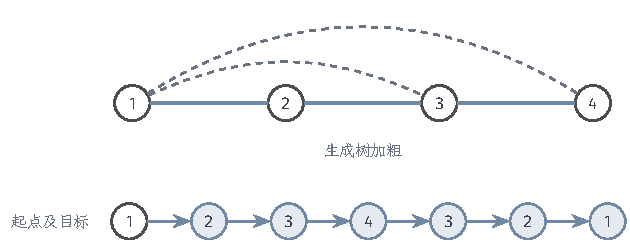
\includegraphics[width=106.726mm]{figures/03-graphs/05-matrices-and-spectra/tikz/walk-examples/cover-tree-targets.pdf}
\caption{用四点环加对角线$\{1,3\}$说明遍历上界。粗实线是所选树边，虚线是原图的其余边。下方从白底的起点$1$开始，箭头依次指向六个等待目标。实际游走仍可沿原图的所有边转移。}
\label{fig:graph-walk-cover-tree-targets}
\end{BookInlineFigure}

命中当前目标后，棋子的位置已经确定。下一段等待的期望就是从该位置出发的首达期望，与此前走过哪些顶点无关。

按名单完成全部目标时，每个顶点一定都已访问过。实际遍历可能更早结束——某些顶点在正式等到它之前已经顺路走过。因此名单给出的总等待时间是一个上界。

将每条树边的去程和返程配对，利用往返公式~\eqref{eq:graph-walk-commute-time}，得到
\begin{equation}
C_u\le\sum_{\{a,b\}\in T}(h_{a,b}+h_{b,a})
=\operatorname{vol}(V)\sum_{\{a,b\}\in T}R_{a,b}.
\label{eq:graph-walk-cover-resistance}
\end{equation}

每条树边$\{a,b\}$本身已经存在于图中。将全部单位电流送过这条边，可行流的耗散为$1/w_{a,b}$。有效电阻是所有单位流的最小耗散，因此$R_{a,b}\le1/w_{a,b}$。

对无权图，每条树边的$R_{a,b}\le1$，树有$n-1$条边，总加权度为$2m$，于是
\begin{equation}
C\le2m(n-1).
\label{eq:graph-walk-cover-unweighted}
\end{equation}
路径图的$m=n-1$，从端点出发的下界$(n-1)^2$与上界$2(n-1)(n-1)$同阶，因此最坏起点的遍历期望为$\Theta(n^2)$。

\paragraph{三次方量级的构造}

取一个$k$点完全图，在其中一个顶点$u$上接出一条含$\ell$条边的路径，末端为$v$。路径上所有边串联在$u,v$之间，完全图只在$u$处与路径相接，无法分担通往$v$的电流，因此$R_{u,v}=\ell$。

完全图已有$k(k-1)/2$条边，路径增加$\ell$条，每条边两端都计入度数，总加权度为$k(k-1)+2\ell$。

从$v$出发首次到达$u$以前，棋子只能在路径上行走，故$h_{v,u}=\ell^2$。利用往返公式减去这一方向，得
\[
h_{u,v}=\operatorname{vol}(V)\,R_{u,v}-h_{v,u}
=(k(k-1)+2\ell)\ell-\ell^2=k(k-1)\ell+\ell^2.
\]
遍历至少要到达$v$。当$k$与$\ell$都和$n=k+\ell$同阶时，这一项给出$\Theta(n^3)$的下界，与式~\eqref{eq:graph-walk-cover-unweighted}的上界量级一致。大量边集中在一个团里，增加了找到路径入口前的等待。

\section{PageRank}
\label{sec:graph-pagerank}

把网页看成顶点，链接看成有向边。只沿链接行走时，棋子可能进入走不出来的区域，也可能来到没有出边的页面。给行走加入重新选择顶点的机会，可以用长期分布为页面排名。这种做法称为\term{PageRank}\scite{page1999pagerank}。

\subsection{PageRank方程}
\label{sec:graph-pagerank-equation}

\paragraph{有向图的转移矩阵}

有向图的弧只从尾端指向头端。计算顶点$i$的转移概率时，只读取从$i$出去的弧，按出弧权重的总和归一化。

若某个顶点没有出边，就没有权重可以归一化。设$\bm{s}$为给定的概率行，用它补上零出度顶点所在的行。补齐后的$\bm{P}$每行非负、和为一，是一个行随机矩阵。

\paragraph{平稳分布的存在}

有限行随机矩阵总有平稳分布。为说明这一点，取任意概率初态$\bm{\nu}^{(0)}$，把前$T$步的分布取平均，
\[
\bm{a}^{(T)}=\frac{1}{T}\sum_{t=0}^{T-1}\bm{\nu}^{(0)}\bm{P}^t.
\]
右乘$\bm{P}$将每个时刻推进一步，新平均覆盖第$1$到第$T$步。中间$T-1$项相同，首尾两项之差除以$T$趋于零，
\[
\bm{a}^{(T)}\bm{P}-\bm{a}^{(T)}
=\frac{\bm{\nu}^{(0)}\bm{P}^T-\bm{\nu}^{(0)}}{T}
\to\bm{0}.
\]
这些平均都是概率行，位于有限维的闭有界集合中。从中选出一个收敛子列，极限就是平稳分布。

\paragraph{不唯一和振荡}

存在平稳分布之后，还要问它是否唯一、迭代能否收敛到它。

两个互不相连的有向环各有一个平稳分布，初态的分配方式会影响极限。即使平稳解唯一，迭代也可能振荡——一个两点有向环的唯一平稳分布是$(1/2,1/2)$，但从一点出发，分布在两个顶点之间永远交替。

\paragraph{重启机制}

为了同时解决不唯一和振荡，在每一步独立决定是否重启。以概率$\alpha\in(0,1)$按$\bm{s}$选择新位置，以概率$1-\alpha$按补齐后的$\bm{P}$转移。重启这一支不依赖当前位置，总使用同一份$\bm{s}$。

如果当前分布为$\bm{p}$，两支分别向下一步贡献$\alpha\bm{s}$和$(1-\alpha)\bm{p}\bm{P}$。要求下一步仍是$\bm{p}$，得到
\begin{equation}
\bm{p}=\alpha\bm{s}+(1-\alpha)\bm{p}\bm{P}.
\label{eq:graph-pagerank-fixed-point}
\end{equation}

这个方程还有另一种理解方式。先按$\bm{s}$选起点，每到一个位置，以概率$\alpha$结束，否则按$\bm{P}$再走一步。绕过前$t$次结束机会才在第$t+1$次结束，行走恰好走了$t$步，概率为$\alpha(1-\alpha)^t$。终点分布按步数加权求和，得
\begin{equation}
\bm{p}=\alpha\sum_{t=0}^{\infty}(1-\alpha)^t\bm{s}\bm{P}^t.
\label{eq:graph-pagerank-series}
\end{equation}
第零项对应立即结束的$\alpha\bm{s}$。把其余各项整体前移一个步数，提出公因子$(1-\alpha)$和一次$\bm{P}$，恰好得到$(1-\alpha)\bm{p}\bm{P}$。两部分相加满足式~\eqref{eq:graph-pagerank-fixed-point}。

\paragraph{唯一性与收敛性}

对任意两份概率差$\bm{z}$，一步转移不会放大$\ell^1$距离：逐列取绝对值并利用行和为一，$\lVert\bm{z}\bm{P}\rVert_1\le\lVert\bm{z}\rVert_1$。式~\eqref{eq:graph-pagerank-fixed-point}右端的更新映射$F$满足
\begin{equation}
\lVert F(\bm{x})-F(\bm{y})\rVert_1
\le(1-\alpha)\lVert\bm{x}-\bm{y}\rVert_1.
\label{eq:graph-pagerank-contraction}
\end{equation}
这是因为两个输入共享同一份重启$\alpha\bm{s}$，差值只出现在$1-\alpha$比例的转移部分。

若存在两个平稳解，更新后它们不变、距离不变，但收缩系数$1-\alpha<1$迫使距离为零。唯一性得证。从任意初态出发，第$t$轮与真解的距离每轮至少缩小为$1-\alpha$倍，因此迭代收敛。

\subsection{算法实现}
\label{sec:graph-pagerank-implementation}

输入为有向邻接表、概率行$\bm{s}$、重启概率$\alpha$和$\ell^1$误差容限$\varepsilon$。算法维护一份候选排名$\bm{p}^{(t)}$，从$\bm{p}^{(0)}=\bm{s}$开始。每一轮先沿实际出边传播概率，再加上重启部分。

\begin{algorithm}[PageRank迭代]
\label{alg:graph-pagerank-iteration}
输入：有向邻接表、概率行$\bm{s}$、重启概率$\alpha$、容许$\ell^1$误差$\varepsilon$。输出：近似排名$\bm{p}$。
\begin{enumerate}
  \item 令$\bm{p}^{(0)}=\bm{s}$。对零出度顶点记录标志。
  \item 每轮执行更新$\bm{p}^{(t+1)}=\alpha\bm{s}+(1-\alpha)\bm{p}^{(t)}\bm{P}$。实现时：先对每个正出度顶点$i$，把$(1-\alpha)p^{(t)}_i$按出边权重比例分给各头端。同时累计所有零出度顶点上的质量$q$，统一加回$q\bm{s}$。最后再加上重启项$\alpha\bm{s}$。
  \item 计算残差$\bm{r}=\bm{p}^{(t+1)}-\bm{p}^{(t)}$。若$\lVert\bm{r}\rVert_1\le\alpha\varepsilon$，返回$\bm{p}^{(t+1)}$。
\end{enumerate}
\end{algorithm}

每轮更新写成公式为
\begin{equation}
\bm{p}^{(t+1)}=\alpha\bm{s}+(1-\alpha)\bm{p}^{(t)}\bm{P}.
\label{eq:graph-pagerank-iteration}
\end{equation}

每轮先沿实际出边传播概率。对于零出度的顶点，只把它的分数加到悬挂质量$q$中。边扫描结束后，统一把$q\bm{s}$加到尚未乘$1-\alpha$的一步结果中。这等价于给每个悬挂点补上同一行$\bm{s}$，只需存一份重启分布。

考虑四个顶点及单位权弧$1\to2$、$2\to3$、$3\to1$、$3\to4$。顶点$4$没有出边。取$\bm{s}=(1,0,0,0)$、$\alpha=1/2$。每轮的重启部分给顶点$1$增加$1/2$的质量。

第一轮开始时全部质量在$1$，沿边部分的$1/2$送往$2$。第二轮将顶点$1$的质量减半后送到$2$，同时将$2$的质量减半后送到$3$，两点各得$1/4$。第三轮中，顶点$3$的$1/4$里有$1/2$沿边分出，分给$1,4$各$1/16$。这是顶点$4$首次收到质量。各轮结果为
\[
\begin{array}{c@{\qquad}c}
t&\bm{p}^{(t)}\\
1&(1/2,1/2,0,0)\\
2&(1/2,1/4,1/4,0)\\
3&(9/16,1/4,1/8,1/16)\\
4&(9/16,9/32,1/8,1/32)
\end{array}
\]
第四轮中，顶点$4$的旧质量$1/16$通过零出度填补分给顶点$1$，再乘沿边比例$1/2$，贡献$1/32$。同轮$3$也沿弧$3\to1$送来$1/32$。重启的$1/2$加上这两笔，$1$的新质量为$9/16$。图~\ref{fig:graph-pagerank-fourth-round}给出这一轮的各笔转移。

\begin{BookInlineFigure}
\centering
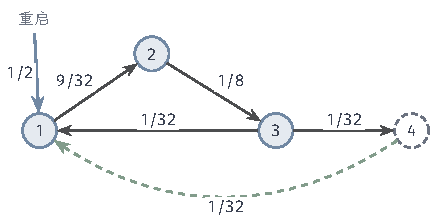
\includegraphics[width=73.459mm]{figures/03-graphs/05-matrices-and-spectra/tikz/walk-examples/pagerank-fourth-round.pdf}
\caption{四页算例在第四轮的质量分配，重启概率为$1/2$，重启集中到顶点$1$。深灰实线沿实际链接送出质量，虚线是零出度顶点$4$补齐后送出的份额。重启直接增加顶点$1$的质量。}
\label{fig:graph-pagerank-fourth-round}
\end{BookInlineFigure}

每轮所得各项非负，总和应为一，可据此检查传播、悬挂补偿和重启项是否漏加。

\subsection{算法分析}
\label{sec:graph-pagerank-cost}

由式~\eqref{eq:graph-pagerank-contraction}及两份概率行的$\ell^1$距离至多为$2$，第$t$轮的误差满足
\begin{equation}
\lVert\bm{p}^{(t)}-\bm{p}\rVert_1\le 2(1-\alpha)^t.
\label{eq:graph-pagerank-geometric-bound}
\end{equation}
要将上界压到$\varepsilon$，对$2(1-\alpha)^t\le\varepsilon$取对数，得到充分的迭代轮数
\[
t\ge \left\lceil\frac{\log(2/\varepsilon)}{-\log(1-\alpha)}\right\rceil.
\]
例如$\alpha=1/2$时，六轮可把上界压到$1/32$。当$\alpha$很小时，$-\log(1-\alpha)$与$\alpha$同阶，轮数约为$\alpha^{-1}\log(2/\varepsilon)$。

在运行中，真解$\bm{p}$未知，但可以计算候选$\bm{q}$再走一轮会变多少。记残差为$\bm{r}=F(\bm{q})-\bm{q}$。从$\bm{q}$到真解$\bm{p}$的距离，可以先走到$F(\bm{q})$再走到$F(\bm{p})=\bm{p}$。第一段距离是$\lVert\bm{r}\rVert_1$，第二段由收缩性控制，因此
\[
\lVert\bm{q}-\bm{p}\rVert_1
\le\lVert\bm{r}\rVert_1+(1-\alpha)\lVert\bm{q}-\bm{p}\rVert_1.
\]
移项得到
\begin{equation}
\lVert\bm{q}-\bm{p}\rVert_1\le\frac{\lVert\bm{r}\rVert_1}{\alpha}.
\label{eq:graph-pagerank-residual-bound}
\end{equation}
若残差范数不超过$\alpha\varepsilon$，当前候选的误差就不超过$\varepsilon$。

设图有$n$个顶点、$m$条弧。每轮传播扫描$m$条弧，初始化和悬挂补偿需$O(n)$。每轮时间和整个存储均为$O(n+m)$。

$\alpha$越大，一次行走越可能很快结束，终点分布越接近$\bm{s}$，迭代也越快收敛。较小的$\alpha$留下更多沿边传播的机会，但也让每轮保留更多旧误差。选择$\alpha$同时改变排名的含义和计算的速度。

\section{个性化PageRank}
\label{sec:graph-personalized-pagerank}

上一节的标准PageRank取均匀跳转分布$\bm s=\frac1n\bm 1^\top$，计算出的是所有节点与查询者无关的“全局通用权威分”。如果我们将重启分布$\bm s$集中到某一个指定节点$u$（或少数几个节点）上，让随机游走每次重启时都回到$u$重新出发，所得的平稳分布就称为\term{个性化PageRank}（personalized PageRank，简称PPR），其中的起点称为\term{种子}（seed）。本节按照“背景与主要思想—算法实现—算法分析”的脉络，介绍个性化PageRank及其在超大规模图上的局部推送算法与局部谱划分应用。

\subsection{背景与主要思想}
\label{sec:graph-pagerank-push-principle}

\paragraph{为什么引入个性化PageRank}

全局排名与针对某个种子的关联排名回答不同的问题。将重启分布集中在顶点$u$后，游走反复从$u$出发，短路径的传播权重通常高于长路径。个性化PageRank由图结构、转移概率与重启概率共同确定，因而可作为相对于种子的关联度量；它不等同于最短路距离，也不保证得分高的顶点一定与种子直接相邻。

第二个问题是如何利用稀疏种子进行局部计算。全局幂迭代通常读取整张图，而局部查询未必需要计算每个顶点的精确分数。重启使长度为$t$的传播项按几何因子衰减，但这不自动保证某个小邻域包含绝大多数概率质量。下面的局部推送通过截断单位度数余量，给出显式的工作量与误差界；在参数和种子支撑较小时，它可能只访问图的一部分。

\paragraph{主要思想：种子重启与局部推送（Local Push）}

本节在至少有两个顶点的连通简单无权图上考察采用惰性转移矩阵$\bm Q=(\bm I+\bm P)/2$的个性化PageRank。在个性化PageRank与局部算法文献中，习惯用$\alpha\in(0,1)$直接表示每一步的\emph{重启（或就地终止）概率}，用$1-\alpha$表示沿惰性矩阵$\bm Q$继续游走一步的概率（对应上一节的阻尼系数$1-\alpha$）。对于任意非负种子向量$\bm s\in\mathbb R^{1\times n}$（通常取单点种子$\bm s=\bm e_u^\top$），对应的个性化PageRank线性算子$\mathcal R(\bm s)$定义为
\begin{equation}
\mathcal{R}(\bm{s})
=\alpha\sum_{t=0}^{\infty}(1-\alpha)^t\bm{s}\bm{Q}^t,
\label{eq:graph-pagerank-linear-operator}
\end{equation}
其满足不动点方程$\mathcal R(\bm s)=\alpha\bm s+(1-\alpha)\mathcal R(\bm s)\bm Q$，且对任意待分配质量行向量$\bm r$满足一步分解恒等式：
\begin{equation}
\mathcal{R}(\bm{r})=\alpha\bm{r}+(1-\alpha)\mathcal{R}(\bm{r}\bm{Q}).
\label{eq:graph-pagerank-push-decomposition}
\end{equation}

如何在不扫描全图的前提下算出$\mathcal R(\bm s)$的高精度近似？Andersen、Chung与Lang于2006年提出了著名的\emph{局部推送}（local push，或ApproximatePR）思想\scite{andersen2006localpagerank}。

其核心设计首先在于\emph{维护“已确认分数$\bm p$ + 待处理余量$\bm r$”的质量守恒不变量}。局部推送不像全局幂法那样每轮同步更新全图所有节点，而是维护两个稀疏行向量：一个是记录已经终止游走、已累积的终点分数的\emph{近似向量}$\bm p$，另一个是记录当前仍滞留在各节点等待继续向外扩散的\emph{余量向量}（residual）$\bm r$。初始时令已确认分数$\bm p=\bm 0$，并将全部初始种子质量放入待处理余量$\bm r=\bm s$。

在每一步局部操作中，算法只单独挑出一个节点$i$，将它当前积压的余量$q=r_i$清空，并按一步分解式~\eqref{eq:graph-pagerank-push-decomposition}拆成两部分处理：其中$\alpha q$比例就地停止游走，直接累加到已确认分数$p_i$中；其余$(1-\alpha)q$比例则按惰性矩阵$\bm Q$向前推进一步，分发给节点$i$自身及它的直接邻居作为新的待处理余量。

由于每次推送只是把单个节点$i$的待处理质量沿着随机游走规则向前推进了一步，整个算法运行期间始终严格保持如下质量守恒不变量：
\begin{equation}
\mathcal{R}(\bm{s})=\bm{p}+\mathcal{R}(\bm{r}).
\label{eq:graph-pagerank-push-invariant}
\end{equation}

对顶点$i$推送一次需读取$d_i$个邻居。用阈值$r_i/d_i>\varepsilon$筛选活跃顶点，便能将每次读取的邻接表大小与被转移到$\bm p$中的质量联系起来。当所有余量均满足$r_i\leq\varepsilon d_i$时停止，可得到逐点误差界。算法不必展开所有顶点的邻接表，但仍会读取被推送顶点的邻居标识并更新余量；是否为亚线性工作量取决于$\alpha,\varepsilon$和种子支撑。

\subsection{算法实现}
\label{sec:graph-pagerank-push-implementation}

\paragraph{局部推送算法步骤}

在简单无权图上，惰性转移矩阵$\bm Q=(\bm I+\bm P)/2$将一半质量留在当前顶点$i$，另一半质量均分给$i$的$d_i$个邻居。因此，对顶点$i$（旧余量记为$q=r_i$）执行一次局部推送的更新公式为
\begin{equation}
\begin{aligned}
p_i &\leftarrow p_i+\alpha q,\\
r_i &\leftarrow (1-\alpha)q/2,\\
r_j &\leftarrow r_j+(1-\alpha)q/(2d_i),\qquad \forall j\sim i.
\end{aligned}
\label{eq:graph-pagerank-push-update}
\end{equation}
采用哈希表（字典）稀疏存储$\bm p$与$\bm r$，并用队列维护满足$r_i>\varepsilon d_i$的活跃顶点，完整算法如下。

\begin{algorithm}[个性化PageRank局部推送（Local Push）]
\label{alg:graph-personalized-pagerank-push}
输入：可按点查询且能常数时间读取度数的无向图邻接表、稀疏种子分布$\bm{s}$、重启概率$\alpha\in(0,1)$、截断阈值$\varepsilon>0$。输出：稀疏近似分数$\bm{p}$与剩余余量$\bm{r}$。
\begin{enumerate}
  \item \textbf{稀疏初始化}：令$\bm{p}=\bm{0}$、$\bm{r}=\bm{s}$。将所有满足$r_i>\varepsilon d_i$的顶点$i$加入活跃队列$Q$。
  \item \textbf{局部推送循环}：当队列$Q$非空时，弹出队首顶点$i$，记其当前余量为$q=r_i$，按式~\eqref{eq:graph-pagerank-push-update}执行局部推送：
    \begin{enumerate}
    \item 划入已确认分数：$p_i\leftarrow p_i+\alpha q$；
    \item 更新本点惰性停留余量：$r_i\leftarrow(1-\alpha)q/2$；
    \item 分发邻居余量：遍历$i$的每个邻居$j\sim i$，令$r_j\leftarrow r_j+(1-\alpha)q/(2d_i)$。
    \end{enumerate}
    更新完毕后，检查顶点$i$及每个邻居$j\sim i$：若某个顶点满足$r_v>\varepsilon d_v$且不在队列$Q$中，将其加入队尾。
  \item \textbf{终止返回}：当队列$Q$为空时停止，返回稀疏向量$\bm{p}$和$\bm{r}$。
\end{enumerate}
\end{algorithm}

\paragraph{四点路径上的三次推送演示}

在单位权四点路径$1\!-\!2\!-\!3\!-\!4$上取单点种子$1$（$\bm s=(1,0,0,0)$），重启概率$\alpha=1/2$，阈值$\varepsilon=1/8$。四个顶点的度依次为$1,2,2,1$，对应的触发阈值$\varepsilon d_i$依次为$\frac18,\frac14,\frac14,\frac18$。
\begin{itemize}
\item \emph{第一次推送顶点$1$}：旧余量$q=1>\frac18$。划入分数$p_1\leftarrow\frac12$；剩余$\frac12$对半分，$r_1\leftarrow\frac14$留在本点，$r_2\leftarrow\frac14$送给邻居$2$，此时$\bm p=(\frac12,0,0,0),\bm r=(\frac14,\frac14,0,0)$。因$r_1=\frac14>\frac18$仍超阈值，顶点$1$继续留在队列中（而$r_2=\frac14$未严格超过$\varepsilon d_2=\frac14$）。
\item \emph{第二次推送顶点$1$}：旧余量$q=\frac14$。划入分数$\frac18$使$p_1=\frac58$；剩余$\frac18$对半分，$r_1\leftarrow\frac{1}{16}$，$r_2\leftarrow\frac14+\frac{1}{16}=\frac{5}{16}$。此时$\bm p=(\frac58,0,0,0),\bm r=(\frac{1}{16},\frac{5}{16},0,0)$，顶点$2$的余量$\frac{5}{16}>\frac14$超过阈值，进入队列。
\item \emph{第三次推送顶点$2$}（图~\ref{fig:graph-pagerank-third-push}）：旧余量$q=\frac{5}{16}$。划入分数$p_2\leftarrow\frac{5}{32}$；剩余$\frac{5}{32}$中一半$\frac{5}{64}$留作$r_2$，另一半$\frac{5}{64}$均分给邻居$1$和$3$（各加$\frac{5}{128}$）。合并后得到
\[
\bm{p}=\left(\frac58,\frac{5}{32},0,0\right),\qquad
\bm{r}=\left(\frac{13}{128},\frac{5}{64},\frac{5}{128},0\right).
\]
此时四个顶点的余量均不再超过各自阈值$\frac18,\frac14,\frac14,\frac18$，队列为空，算法终止。注意最右端的顶点$4$在整个运行过程中从未被访问过（$p_4=r_4=0$）。图~\ref{fig:pagerank-push-evolution}以柱状图直观展示了三次推送中$\bm p$与$\bm r$的消长过程。
\end{itemize}

\begin{BookInlineFigure}
\centering
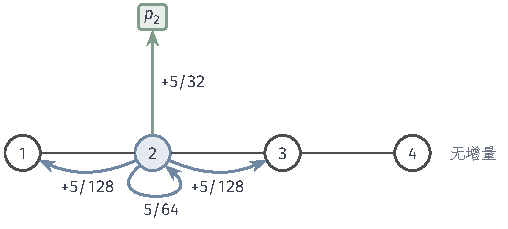
\includegraphics[width=85.965mm]{figures/03-graphs/05-matrices-and-spectra/tikz/walk-examples/pagerank-push-path.pdf}
\caption{四顶点路径上的第三次局部推送（$\alpha=1/2$）。从顶点$2$取出旧余量$5/16$：向上箭头将$5/32$确认为终点分数$p_2$，回环将$5/64$留作本点余量，左右箭头向邻居$1,3$各分发$5/128$余量。}
\label{fig:graph-pagerank-third-push}
\end{BookInlineFigure}

\begin{figure}[!htb]
\centering
\begin{tikzpicture}[x=1mm,y=1mm,
  pbar/.style={fill=FigureBlueFill,draw=FigureBlue,line width=.4pt},
  rbar/.style={fill=FigureYellowFill,draw=FigureYellow,line width=.4pt},
  panel/.style={anchor=mid,font=\figurefont\footnotesize},
  vlabel/.style={font=\figurefont\fontsize{6.5}{8}\selectfont,FigureInk,anchor=north},
  plabel/.style={font=\figurefont\fontsize{6}{7.5}\selectfont,FigureInk,anchor=south}]
  \def\bw{2.6}
  \def\sc{32}
  \def\gp{1.2}
  \def\vgp{3.0}
  \fill[pbar] (0,27) rectangle +(3,2); \node[font=\figurefont\fontsize{6.5}{8}\selectfont,anchor=west] at (4,28) {分数$p_i$};
  \fill[rbar] (20,27) rectangle +(3,2); \node[font=\figurefont\fontsize{6.5}{8}\selectfont,anchor=west] at (24,28) {余量$r_i$};
  \begin{scope}[xshift=0mm]
    \draw[FigureStroke,line width=.35pt] (0,0) -- (0,\sc*0.55);
    \draw[FigureStroke,line width=.35pt] (0,0) -- (4*2*\bw+4*\gp+3*\vgp+1,0);
    \foreach \i/\v/\pv/\rv in {0/1/0.5/0.25, 1/2/0/0.25, 2/3/0/0, 3/4/0/0} {
      \pgfmathsetmacro{\x}{\i*(2*\bw+\gp+\vgp)+1}
      \pgfmathsetmacro{\hp}{\pv*\sc}
      \pgfmathsetmacro{\hr}{\rv*\sc}
      \pgfmathparse{\pv>0?1:0}\ifnum\pgfmathresult=1
        \fill[pbar] (\x,0) rectangle +(\bw,\hp);
      \fi
      \pgfmathparse{\rv>0?1:0}\ifnum\pgfmathresult=1
        \fill[rbar] (\x+\bw+\gp,0) rectangle +(\bw,\hr);
      \fi
      \node[vlabel] at (\x+\bw+\gp/2,-1) {$\v$};
    }
    \node[panel] at (15,-7) {(a) 第$1$次推送后};
  \end{scope}
  \begin{scope}[xshift=36mm]
    \draw[FigureStroke,line width=.35pt] (0,0) -- (0,\sc*0.7);
    \draw[FigureStroke,line width=.35pt] (0,0) -- (4*2*\bw+4*\gp+3*\vgp+1,0);
    \foreach \i/\v/\pv/\rv in {0/1/0.625/0.0625, 1/2/0/0.3125, 2/3/0/0, 3/4/0/0} {
      \pgfmathsetmacro{\x}{\i*(2*\bw+\gp+\vgp)+1}
      \pgfmathsetmacro{\hp}{\pv*\sc}
      \pgfmathsetmacro{\hr}{\rv*\sc}
      \pgfmathparse{\pv>0?1:0}\ifnum\pgfmathresult=1
        \fill[pbar] (\x,0) rectangle +(\bw,\hp);
      \fi
      \pgfmathparse{\rv>0?1:0}\ifnum\pgfmathresult=1
        \fill[rbar] (\x+\bw+\gp,0) rectangle +(\bw,\hr);
      \fi
      \node[vlabel] at (\x+\bw+\gp/2,-1) {$\v$};
    }
    \node[panel] at (15,-7) {(b) 第$2$次推送后};
  \end{scope}
  \begin{scope}[xshift=72mm]
    \draw[FigureStroke,line width=.35pt] (0,0) -- (0,\sc*0.7);
    \draw[FigureStroke,line width=.35pt] (0,0) -- (4*2*\bw+4*\gp+3*\vgp+1,0);
    \foreach \i/\v/\pv/\rv in {0/1/0.625/0.1016, 1/2/0.1563/0.0781, 2/3/0/0.0391, 3/4/0/0} {
      \pgfmathsetmacro{\x}{\i*(2*\bw+\gp+\vgp)+1}
      \pgfmathsetmacro{\hp}{\pv*\sc}
      \pgfmathsetmacro{\hr}{\rv*\sc}
      \pgfmathparse{\pv>0?1:0}\ifnum\pgfmathresult=1
        \fill[pbar] (\x,0) rectangle +(\bw,\hp);
      \fi
      \pgfmathparse{\rv>0?1:0}\ifnum\pgfmathresult=1
        \fill[rbar] (\x+\bw+\gp,0) rectangle +(\bw,\hr);
      \fi
      \node[vlabel] at (\x+\bw+\gp/2,-1) {$\v$};
    }
    \node[panel] at (15,-7) {(c) 第$3$次推送后};
  \end{scope}
\end{tikzpicture}
\caption{四点路径上三次局部推送后的已确认分数$\bm{p}$（蓝色）与待处理余量$\bm{r}$（黄色）。每次推送仅在局部更新被推顶点及其邻居，远端顶点$4$始终未被触及。}
\label{fig:pagerank-push-evolution}
\end{figure}

\subsection{算法分析}
\label{sec:graph-pagerank-push-analysis}

下面证明局部推送的邻接表访问总量与逐点误差界。推送部分的工作量为$O(1/(\alpha\varepsilon))$，另需读取并初始化种子向量的非零支撑；该上界不显式含$n,m$，但参数随图规模变化时并不保证亚线性。局部划分的质量还需要额外的种子和参数条件。

\begin{theorem}[局部推送算法的复杂度与逐点误差界]
\label{thm:graph-pagerank-push-guarantee}
设在连通简单无权图上对非负种子行向量$\bm s$（$\lVert\bm s\rVert_1\leq 1$）、重启概率$\alpha\in(0,1)$和阈值$\varepsilon>0$运行算法~\ref{alg:graph-personalized-pagerank-push}。则算法必在有限步内停止，且满足：
\begin{enumerate}
  \item \emph{总工作量与支撑集上界}：整个运行过程中所有推送操作访问的邻接表边数总和（及已确认分数$\bm p$的非零支撑集体积）满足
  \begin{equation}
  \operatorname{vol}\bigl(\operatorname{supp}(\bm p)\bigr)
  \le \sum_{\text{各次推送}\;i}d_i
  \le \frac{\lVert\bm s\rVert_1}{\alpha\varepsilon}
  \le \frac{1}{\alpha\varepsilon}.
  \label{eq:graph-pagerank-push-work}
  \end{equation}
  \item \emph{逐点相对度数误差与总质量守恒}：算法停止时输出的$(\bm p,\bm r)$对全图每个顶点$i\in V$满足
  \begin{equation}
  0\le\mathcal{R}(\bm{s})_i-p_i\le\varepsilon d_i,
  \qquad
  \frac{\mathcal{R}(\bm s)_i}{d_i} - \varepsilon \le \frac{p_i}{d_i} \le \frac{\mathcal{R}(\bm s)_i}{d_i},
  \label{eq:graph-pagerank-push-pointwise}
  \end{equation}
  且$\ell^1$总误差恒等于剩余余量的总质量：
  \begin{equation}
  \lVert\mathcal{R}(\bm{s})-\bm{p}\rVert_1=\lVert\bm{r}\rVert_1.
  \label{eq:graph-pagerank-push-mass}
  \end{equation}
\end{enumerate}
\end{theorem}

\begin{proof}
（1）每次从队列中弹出顶点$i$执行推送时，该点必满足触发条件$q=r_i>\varepsilon d_i$。此次推送将$\alpha q>\alpha\varepsilon d_i$的质量从余量$\bm r$转化为已确认分数$\bm p$，而其余$(1-\alpha)q$的质量只是在余量向量内部重新分配，因此余量总和$\lVert\bm r\rVert_1$在此次推送中净减少$\alpha q>\alpha\varepsilon d_i$。由于初始余量总和为$\lVert\bm s\rVert_1\leq 1$且余量始终非负，全部推送操作累计减少的余量不可能超过$\lVert\bm s\rVert_1$：
\[
  \sum_{\text{各次推送}\;i}\alpha\varepsilon d_i \leq \sum_{\text{各次推送}\;i}\alpha q \leq \lVert\bm s\rVert_1\leq 1.
\]
由于每个顶点的度至少为$1$，每次推送至少减少$\alpha\varepsilon$的余量，因此推送次数有限。两边同除以$\alpha\varepsilon$即得式~\eqref{eq:graph-pagerank-push-work}（每个$p_i>0$的顶点至少被推送过一次，故$\operatorname{vol}(\operatorname{supp}(\bm p))\leq\sum d_i\leq\frac{1}{\alpha\varepsilon}$）。

（2）算法停止时队列为空，说明每个顶点$i\in V$的剩余余量均满足$0\leq r_i\leq\varepsilon d_i$，即逐分量有$\bm 0^\top\leq\bm r\leq\varepsilon\bm d^\top$。在无向图上，由详细平衡知度向量满足$\bm d^\top\bm P=\bm d^\top$，从而在惰性矩阵$\bm Q=(\bm I+\bm P)/2$下同样满足平稳性$\bm d^\top\bm Q=\bm d^\top$。因为$\bm Q$的元素全部非负，右乘$\bm Q^t$保持逐分量不等号方向：
\[
  \bm 0^\top\leq\bm r\bm Q^t\leq\varepsilon\bm d^\top\bm Q^t=\varepsilon\bm d^\top\qquad(\forall t\geq 0).
\]
代入级数定义~\eqref{eq:graph-pagerank-linear-operator}并结合守恒不变量~\eqref{eq:graph-pagerank-push-invariant}的$\mathcal R(\bm s)-\bm p=\mathcal R(\bm r)$，立得
\[
  \bm 0^\top\leq\mathcal R(\bm s)-\bm p=\alpha\sum_{t=0}^\infty(1-\alpha)^t\bm r\bm Q^t\leq\alpha\sum_{t=0}^\infty(1-\alpha)^t\varepsilon\bm d^\top=\varepsilon\bm d^\top,
\]
取第$i$个分量即为式~\eqref{eq:graph-pagerank-push-pointwise}。最后，因$\mathcal R(\bm r)\geq\bm 0^\top$且算子$\mathcal R$保持向量分量和不变，有$\lVert\mathcal R(\bm s)-\bm p\rVert_1=\lVert\mathcal R(\bm r)\rVert_1=\lVert\bm r\rVert_1$。
\end{proof}

\paragraph{基于个性化PageRank的局部谱划分}

定理~\ref{thm:graph-pagerank-push-guarantee}给出的一个结论是式~\eqref{eq:graph-pagerank-push-pointwise}第二式：局部推送得到的单位度数分数$p_i/d_i$是对真实平稳概率比$\mathcal R(\bm s)_i/d_i$的$\varepsilon$一致逼近，且非零支撑集$S_+=\{i\in V:p_i>0\}$的体积至多为$\frac{1}{\alpha\varepsilon}$。

在全图体积已给定的前提下，这使我们能够将第~\ref{chap:spectral-partition}章的阈值扫描搬到种子附近的候选顶点集$S_+$上（割权与体积仍按原图计算，不能丢弃通向$V\setminus S_+$的边）：只需将满足$p_i>0$的少量顶点按归一化分数$p_i/d_i$从大到小排序，依次扫描非空且不等于全图的前缀集合，并选出导通率$\phi(S)$最小的切分（耗时为$O(\frac{1}{\alpha\varepsilon}\log n)$）。

例如在两个三角形$\{1,2,3\}$与$\{4,5,6\}$经桥边$\{3,4\}$相连的杠铃图上，取$\alpha=1/5,\varepsilon=1/25$，从种子$1$出发执行局部推送后仅顶点$1,2,3$获得正分数，按$p_i/d_i$排序扫描出的前缀$\{1,2,3\}$直接命中了导通率$\phi=1/7$的左团瓶颈割。

这一算例不构成对任意种子和参数的质量保证。Andersen、Chung与Lang的局部划分结果还要求种子属于目标集合中的良种子集，并按目标导通率选择重启概率、截断精度及体积尺度\scite{andersen2006localpagerank}。

原文的精确PageRank扫描保证与带体积筛选的PageRank-Nibble算法是不同结果：后者在给定目标导通率$\varphi$和尺度$2^b$时具有$O(2^b\log^3 m/\varphi^2)$的运行时间界，目标集合还须满足相应的导通率与体积条件。不能将其直接归结为本节任意参数下的局部推送保证。

\section{本章小结}
\label{sec:graph-walk-summary}

本章以图上的随机游走为主线，将前几章建立的矩阵幂、归一化拉普拉斯谱、Cheeger导通率以及电网络有效电阻融会贯通。

在位置分布与混合速度方面，随机游走的一步转移规则由行随机矩阵$\bm P=\bm D^{-1}\bm W$描述，多步分布由$\bm\nu^{(t)}=\bm\nu^{(0)}\bm P^t$给出。无向连通图的详细平衡与拉普拉斯零空间保证了按度数分配的平稳分布$\pi_i=d_i/\operatorname{vol}(V)$唯一存在。

通过度平方根相似变换$\bm S=\bm D^{1/2}\bm P\bm D^{-1/2}=\bm I-\mathcal L$，从任意初始分布出发均收敛于$\bm\pi$当且仅当图不是二部图（$\theta_n>-1$）；引入惰性游走$\bm Q=(\bm I+\bm P)/2$可消除负特征值奇偶振荡，使非平稳谱模长由$\gamma=\mu_2/2$决定，具体误差界还含初态因子，并经由Cheeger不等式$\phi_*^2/4\leq\gamma\leq\phi_*$与图的瓶颈导通率$\phi_*$紧密相连。

在首达时间方面，不同起终点间的最大期望在完全图（$\Theta(n)$）、路径与环（$\Theta(n^2)$）、超立方体（$\Theta(n)$）以及棒棒糖图（$\Theta(n^3)$）中展示了不同的等待时间量级。一般图上首达期望满足接地拉普拉斯方程$\bm L_{-j,-j}\bm h_{-j,j}=\bm d_{-j}$，而两点间的往返时间则满足电学恒等式$h_{i,j}+h_{j,i}=\operatorname{vol}(V)R_{i,j}$，对连通简单单位权图，由此得到首达时间上界$2m\,\operatorname{dist}(i,j)\leq 2m(n-1)<n^3$。

进一步，Matthews定理通过调和数$H_{n-1}$将遍历时间$C$夹在$h_{\min}H_{k-1}$与$h_{\max}H_{n-1}$之间，而生成树深度优先巡游则利用有效电阻给出了消除多余对数因子的遍历上界$C\leq\operatorname{vol}(V)\sum_{e\in T}R_e$，在单位权图上进一步有$C\leq2m(n-1)$。

在有向图PageRank中，死胡同修补与阻尼跳转给出唯一平稳分布；只有跳转分布处处为正时，才直接保证所有顶点得分严格为正。非平稳特征值模长不超过阻尼系数$\alpha$，稀疏幂法具有几何收缩界与残差误差证书。

个性化PageRank一节改用$\alpha$表示重启概率：局部推送在不变量$\mathcal R(\bm s)=\bm p+\mathcal R(\bm r)$下具有$O(1/(\alpha\varepsilon))$的推送工作量和单位度数误差界，另需种子初始化成本。它是否为亚线性算法取决于参数；局部切分还需排序、按原图计算割权，以及额外的种子与质量保证条件。

